\documentclass{sig-alternate-05-2015}

\usepackage{xcolor}
\usepackage{multicol}
\usepackage{stackengine}
\usepackage{bussproofs}
\newcommand{\lab}[1]{\RightLabel{\textsc{\small #1}}}
\newenvironment{bpt}{\leavevmode\hbox\bgroup}{\DisplayProof\egroup}
\usepackage[final]{listings}

\lstdefinelanguage{JavaScript}{
  keywords={typeof, new, true, false, catch, function, return, null, catch, switch, var, if, in, while, do, else, case, break, fx},
  keywordstyle=\color{blue}\bfseries,
  ndkeywords={class, export, boolean, throw, implements, import, this},
  ndkeywordstyle=\color{darkgray}\bfseries,
  identifierstyle=\color{black},
  sensitive=false,
  comment=[l]{//},
  morecomment=[s]{/*}{*/},
  commentstyle=\color{purple}\ttfamily,
  stringstyle=\color{red}\ttfamily,
  morestring=[b]',
  morestring=[b]"
}
\lstset{language=JavaScript,
        basicstyle=\ttfamily\small,
        aboveskip={0.5\baselineskip},
        belowskip={0.5\baselineskip},
        showstringspaces=false,
        captionpos=b}

\usepackage{tikz}
\usetikzlibrary{trees,automata,positioning,arrows}
\tikzstyle{box} = [rounded corners, draw=black, thick, fill=none, text centered, minimum height=6mm,minimum width=12mm]

\begin{document}

% Copyright
\setcopyright{acmcopyright}
%\setcopyright{acmlicensed}
%\setcopyright{rightsretained}
%\setcopyright{usgov}
%\setcopyright{usgovmixed}
%\setcopyright{cagov}
%\setcopyright{cagovmixed}


% DOI
\doi{10.475/123_4}

% ISBN
\isbn{123-4567-24-567/08/06}

%Conference
\conferenceinfo{CROW '16}{March 14--17, 2016, Malaga, Spain}

\acmPrice{\$15.00}

\title{Syntax Extension for Reactive Variables}
\subtitle{Short Paper}

\numberofauthors{2}

\author{
% 1st. author
\alignauthor Christopher Schuster\\
       \affaddr{University of California}\\
       \affaddr{Santa Cruz}\\
       \email{cschuste@ucsc.edu}
% 2nd. author
\alignauthor Cormac Flanagan\\
       \affaddr{University of California}\\
       \affaddr{Santa Cruz}\\
       \email{cormac@ucsc.edu}
}

\maketitle
\begin{abstract}
  Reactive Programming enables the declarative definition of time-variant values (signals) and their dependencies in a way that changes are automatically propagated along the edges of the resulting signal graph.  In order to use reactive programming in an imperative, object-oriented programming language, these signals could be modelled with special data structures.  However, computations on primitive values then have to lifted to signals which usually involves verbose notation.


  This paper introduces \emph{reactive variables} as a syntactic extension for reactive programming.  References to reactive variables always denote their latest values which simplifies mapping and composing of signals.  In order to preserve the correct change propagation semantics, reactive variables have a separate scope from regular variables.  Additionally, we present a working prototype implementation for reactive variables in JavaScript based on the sweet.js macro system.
\end{abstract}

%
% The code below should be generated by the tool at
% http://dl.acm.org/ccs.cfm
% Please copy and paste the code instead of the example below.
%
\begin{CCSXML}
<ccs2012>
<concept>
<concept_id>10011007.10011006.10011008.10011009</concept_id>
<concept_desc>Software and its engineering~Language types</concept_desc>
<concept_significance>500</concept_significance>
</concept>
<concept>
<concept_id>10011007.10011006.10011008.10011024</concept_id>
<concept_desc>Software and its engineering~Language features</concept_desc>
<concept_significance>500</concept_significance>
</concept>
</ccs2012>
\end{CCSXML}

\ccsdesc[500]{Software and its engineering~Language types}
\ccsdesc[500]{Software and its engineering~Language features}

\printccsdesc

\keywords{Reactive Programming, Syntactic Extension, JavaScript}

\section{Introduction}

Reactive Programming is a programming paradigm which has recently attracted more attention due to its benefits for programming user interfaces.  In contrast to imperative programming languages, reactive languages do not evaluate a program statement by statement.  Instead, values are recomputed whenever their inputs are updated.  Thereby, the program becomes a \emph{signal graph} in which change is propagated along edges in which the nodes are \emph{signals}, i.e. values that change over time.  An advantage of this programming paradigm over imperative execution is that updates do not have to be manually triggered and dependencies can be written as \emph{unidirectional constraints}.

One challenge of reactive programming is the integration with imperative code.  While libraries can provide data structures for creating signal graphs with reactive change propagation, these library often require code to be lifted onto signals which involves significant syntactic overhead.

This paper proposes a syntactic extension which introduces first-class \emph{reactive variables} whose scope is separated from regular variables and which are updated using reactive programming semantics.

This extension was implemented for JavaScript using the sweet.js macro system and would be compatible with existing libraries for reactive programming while enabling a more declarative syntax.  Additionally, this paper also includes a concise definition of formal semantics for reactive variables which would be applicable to any programming with extensible syntax like a macro system.

To summarize, this short paper

\begin{itemize}
  \item proposes a new syntactic extension called \emph{reactive variable},
  \item describes an implementation for JavaScript based on the sweet.js macro system, and
  \item formalizes this extension for a simple lambda calculus.
\end{itemize}

\section{Existing Approach}

To motivate the need for reactive programming, let us consider a common use case of an interactive application whose output depends on multiple sources of events.

\subsection{Imperative Updates}

The JavaScript application shown in Figure \ref{lst:imperative} implements a counter which can be paused and resumed with a button which is also used to show the current count.  There are two sources of change: a regular event which is triggered every 100 milliseconds and button clicks by the user.  These two events are handled with callbacks which modify variables and update the user interface.

\begin{figure}
  \begin{lstlisting}
 1 var count = 0, counting = true;
 2 setInterval(function() {
 3   if (counting) {
 4     count++;
 5     $(countBtn).text('Count: ' + count);
 6   }
 7 }, 100);
 8 $(countBtn).click(function() {
 9   counting = !counting;
10   $(countBtn).text(
11     counting ? "Count: " + count : "Paused");
12 });\end{lstlisting}
\caption{Traditional JavaScript code with callback and imperative updates.}
\label{lst:imperative}
\end{figure}

This imperative approach has the main disadvantages that dependent state needs to be updated manually upon changes to either of the two variables which results in code duplication as seen on lines 5 and 10-11.

\subsection{Reactive Programming Libraries}

Interactive applications with user interfaces often involve reactive state updates that depend on events.  Therefore, it benefits from reactive programming which automatically propagates changes.  A common approach to enable reactive programming in an imperative language is to use a library with data structures for creating signals, combining signals and lifting primitive operations onto signals.

The code in Figure \ref{lst:rxjs} illustrates how the code in Figure \ref{lst:imperative} could be rewritten with the RxJS library\footnote{\texttt{https://github.com/Reactive-Extensions/RxJS}} for reactive extensions in JavaScript.  Here, \lstinline+countingSignal+ is a signal of boolean values, denoting whether the program is counting at each point in time.  Starting with an initial value of \lstinline+true+, every click on the button causes the value to flip.  The second signal is based on sampling every 100 milliseconds, will be paused depending on the first signal and otherwise increments a counter starting with 0.  The \lstinline+combineLatest+ methods allows both signal to be combined in a way that any change change in one of the values results in a new string which will be used as label for the button.

\begin{figure}
\begin{lstlisting}
 1 var countingSignal = Rx.Observable
 2   .fromEvent($("#countBtn"), "click")
 3   .scan(function(cnt) { return !cnt; }, true)
 4   .startWith(true);
 5 Rx.Observable
 6   .interval(100)
 7   .pausable(countingSignal)
 8   .scan(function(c) { return c + 1; }, 0)
 9   .startWith(0)
10   .combineLatest(countingSignal,
11     function(count, counting) {
12       return counting
13              ? "Count: " + count
14              : "Paused"; })
15   .subscribe(function(s) {
16     $("#countBtn").text(s); });\end{lstlisting}
\caption{Using the RxJS library for Functional Reactive Programming.}
\label{lst:rxjs}
\end{figure}

Compared to the standard imperative approach, the reactive programming library allows a more declarative solution.  In particular, the \lstinline+combineLatest+ method for combining two signals is preferable to manual state updates, as it ensures that any update is always propagated and the subsequent step to update the user interface in lines 12-14 does not need to be duplicated.

The main disadvantage of the solution shown in Figure \ref{lst:rxjs} is the notation to express the signal graph which involves many cascaded method calls.  The actual computation cannot operate on signals directly, instead the programmer writes functions that operate on primitive values and passes these functions to the library in order to lift the primitive computation to the level of a signal.  Essentially, signals are second-class citizens when using a library approach for reactive programming in JavaScript.

\section{Reactive Variables}

While syntactic extensions with macros are quite common in Languages like Lisp and Scheme, adoption of macros in modern object-oriented languages has been slow; partly due to problems and limitations of string-based macros in C and C++.  However, a light-weight syntactic extension with a macro could support reactive programming and lift the drawbacks of reactive programming libraries which are mainly caused by their syntactic overhead.

Signals, i.e. state that changes reactively depending on events or other parts of the state, behave different from regular variables.  For example, it should not be possible to write to a signal and immediately read from it before the change has been propagated to dependent state.  At the same time, it is possible to write simple expressions that reference signals and simply combine their latest values using standard evaluation semantics.

Therefore, we propose to add a \lstinline+rlet+ language construct which introduces \emph{reactive variables}.  These allow programmers to hide the underlying signal data structure and treat the variable as holding a primitive value.  However, in order to guarantee change propagation and reactive programming semantics, reactive variables can only be referenced by other reactive variables or subscribed to with asynchronous callbacks.  This means that reactive variables have a separate scope from regular variables.
% Additionally, reactive variables cannot be reassigned, which also ensures that there are no cyclic dependencies between reactive variables.

% \begin{figure}
% \begin{lstlisting}
% 1 rlet count = subscribe(interval(100))
% 2              initially(0) count + 1;
% 3 rlet clicks = subscribe($(countBtn).click);
% 4 rlet counting = subscribe(clicks)
% 5                 initially(false) !counting;
% 6 rlet txt =
% 7   counting ? "Count: " + count : "Paused";
% 8 subscribe(txt) { $("#countBtn").text(txt); }\end{lstlisting}
% \caption{First-class reactive variables with \texttt{rlet}.}
% \label{lst:rlet}
% \end{figure}

\begin{figure}
\begin{lstlisting}
1 rlet counting = subscribe($(countbtn).click)
2                 initially(false) !counting;
3 rlet count = subscribe(interval(100))
4              initially(0)
5              counting ? count + 1 : count;
6 rlet txt =
7   counting ? "Count: " + count : "Paused";
8 subscribe(txt) { $("#countBtn").text(txt); }\end{lstlisting}
\caption{First-class reactive variables with \texttt{rlet}.}
\label{lst:rlet}
\end{figure}

\subsection{Types of Change Propagation}
\label{ssec:req}

There could be many different alternative syntax options for defining reactive variables.  Regardless of the concrete choice of keywords and delimiters, any syntax for reactive variables should support at least the following four ways of propagating changes:

\begin{enumerate}
  \item simple expressions which can reference other reactive variables \\ (e.g. \lstinline|rlet c = a + b|),
  \item reactive variables that subscribe to imperative events or callbacks \\ (e.g. \lstinline|rlet clicks = subscribe(button.click)|),
  \item imperative code snippets which are invoked in response to changes of a reactive variable \\ (e.g. \lstinline|subscribe(c) { alert(c); }|), and
  \item a way for reactive variables to access its previous values and have an explicit initial value \\ (e.g. \lstinline|rlet c = initially(0) a + c; }|).
\end{enumerate}

Essentially, the first features enables change propagation between reactive variables, the second feature allows introduces change events from the imperative programming context, the third feature allows reactive updates to trigger imperative execution and the fourth features enables reactive variables to be stateful which corresponds to a \lstinline+fold+ or \lstinline+scan+ of the signal.

\subsection{Proposed Syntax}

The example code in Figure \ref{lst:rlet} illustrates how reactive variables as syntax extension support reactive programming.  The example uses all four features described in the previous section which can also be seen in its signal graph which is shown in Figure \ref{fig:graph}.

\begin{figure}
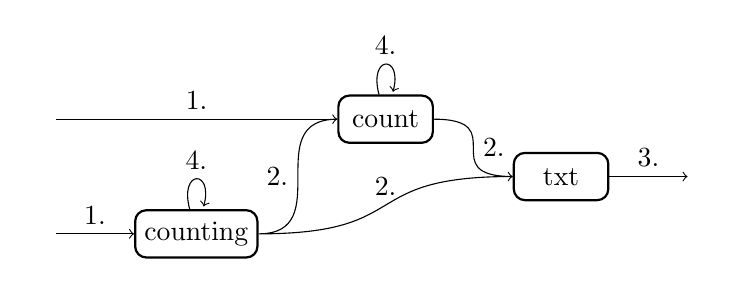
\begin{tikzpicture}
\matrix[row sep=1mm,column sep=10mm] {
  \node (interval) {}; & & \node[box](count){\lstinline+count+}; \\
                       & & & \node[box](txt){\lstinline+txt+}; & \node (text) {}; \\
  \node (clicks) {}; & \node[box](counting){\lstinline+counting+}; \\
};
\path[->,draw] (interval) edge node[above] {1.} (count)
               (count) edge[loop above] node[above] {4.} (count)
               (clicks) edge node[above] {1.} (counting)
               (counting) edge[loop above] node[above] {4.} (counting)
               (counting.east) .. controls +(1,0) and +(-1,0) .. node[left] {2.} (count.west)
               (count.east) .. controls +(1,0) and +(-1,0) .. node[right] {2.} (txt.west)
               (counting.east) .. controls +(2,0) and +(-2,0) .. node[above] {2.} (txt.west)
               (txt) edge node[above] {3.} (text);
\end{tikzpicture}
\caption{Signal graph for reactive variables shown in Figure \ref{lst:rlet}.  The numbers denote the feature used for change propagation (see Section \ref{ssec:req})}
\label{fig:graph}
\end{figure}

Two new language constructs have been added to the JavaScript language which are both used in the example.  Reactive variables can be introduced with \lstinline+rlet+.

\begin{lstlisting}
rlet IDENT = [ subscribe( IDENT|EXPR , ... ) ]
             [ initially( EXPR ) ]
             [ EXPR ]\end{lstlisting}

The optional \lstinline+subscribe( )+ notation allows the newly introduced variable to depend either on other reactive variables which have to be identifiers (change propagation 2.) or on explicit signal values which are passed from the imperative programming context as regular expression at the time the reactive variable gets defined (change propagation 1.).

Another optional part of the definition \lstinline+initially( )+ allows to programmer to define an initial value which is particularly useful if the defining expression references the variable (change propagation 4).

If the variable definition includes a subscription then expression at the end can be omitted and the variable will simply use values as provided by the last subscribed signal.  Otherwise, the expression is the most important part at it describes how the variables is updated and will automatically be reevaluated in response to changed source signals.  With the exception of the subscription, this is the only part of the code that can reference other reactive variables that are in scope (change propagation 2).  Every variables referenced this way is implicitly part of the subscription.

It is important to note that evaluating the primary expression should not involve mutation of global state.  Instead, an additional language construct is provided to execute regular imperative code in response to changes of reactive variables.

\begin{lstlisting}
subscribe ( IDENT , ... ) { STMT ... }\end{lstlisting}

The code is executed asynchronously which also enables asynchronous signal updates (e.g. as part of a network request like \lstinline|rlet res = ajaxGet("/load/" +id) + b|)\footnote{Support for asynchronous signal updates is a desirable features of reactive programming libraries but an orthogonal issue to the addition of syntax extensions for reactive variables.}.

\section{Implementation}



We implemented the syntax extension

based on sweet.js~\cite{disney2014}

\section{Formalism}

\begin{figure*}
  \[\begin{array}{rl}
    v &:= prim ~|~ \lambda x. e ~|~l \hspace{4em} (v: \text{Value},~x: \text{Regular Variable},~r: \text{Reactive Variable},~e: \text{Expression},~l: \text{Location}) \\[1ex]
    e &:= v~|~x~|~r~|~e(e)~|~\text{ref}~e~|~e:=e~|~!e~|~\text{rlet}~r = \text{subscribe}(r...)~\text{initially}(e)~e~\text{in}~e~|~\text{publish} (r,~e)~|~\text{subscribe} (r,e) \\[1ex]
    \multicolumn{2}{l}{
      S~:~r \rightarrow \langle e, l \rangle ~~~~(\text{Signals}) \hspace{4em}
      H ~:~l \rightarrow v ~~~~(\text{Heap}) \hspace{4em}
      R ~:~\mathcal{P}(r)~~~~(\text{Changed reactive variables})} \\[1ex]
    \multicolumn{2}{l}{
    E[\circ] = \circ ~|~ E(e) ~|~ v(E) ~|~ E;e ~|~ \text{ref}~E ~|~ E := e ~|~ l := E ~|~ !E ~|~ \text{publish}(r, E) ~~~~(\text{Evaluation context})} \\
  \end{array}\]

  \textbf{Pure computation ($H,e \rightarrow e$)}

  \begin{center}
  \begin{bpt}
    \AxiomC{~}
    \lab{e-app}
    \UnaryInfC{$H, (\lambda x. e) (v) \rightarrow e[x/v]$}
  \end{bpt} \hspace{1em}
  \begin{bpt}
    \AxiomC{~}
    \lab{e-seq}
    \UnaryInfC{$H, v ; e \rightarrow e$}
  \end{bpt} \hspace{1em}
  \begin{bpt}
    \AxiomC{$H(l) = v$}
    \lab{e-deref}
    \UnaryInfC{$H, !l \rightarrow v$}
  \end{bpt} \\[1ex]
  \end{center}

  \textbf{Imperative evaluation ($S,H,e \twoheadrightarrow H,e$)}

  \begin{center}
  \begin{bpt}
    \AxiomC{$S,H,e \twoheadrightarrow H', e'$}
    \lab{i-ctx}
    \UnaryInfC{$S, H, E[e] \twoheadrightarrow H', E[e']$}
  \end{bpt} \hspace{0em}
  \begin{bpt}
    \AxiomC{$H, e \rightarrow e'$}
    \lab{i-pure}
    \UnaryInfC{$S, H, e \twoheadrightarrow H, e'$}
  \end{bpt} \hspace{0em}
  \begin{bpt}
    \AxiomC{$l~$ fresh $~~H' = H[l := v]$}
    \lab{i-ref}
    \UnaryInfC{$S,H, \text{ref}~v \twoheadrightarrow H', l$}
  \end{bpt} \hspace{0em}
  \begin{bpt}
    \AxiomC{$H' = H[l := v]$}
    \lab{i-asg}
    \UnaryInfC{$S,H, l := v \twoheadrightarrow H', v$}
  \end{bpt} \\[1em]

  \begin{bpt}
    \AxiomC{$l~$ fresh}
    \AxiomC{$S' = S[r := \langle e_3[r/!l], l \rangle]$}
    \AxiomC{$S',H, l := e_i ; e_3 \twoheadrightarrow^{*} H', v$}
    \lab{i-rlet}
    \TrinaryInfC{$S, H, \text{rlet}~r = \text{subscribe}(r...)~\text{initially}(e_i)~e_2~\text{in}~e_3 \twoheadrightarrow H', v$}
  \end{bpt} \\[1em]

  \begin{bpt}
    \AxiomC{$S(r) = \langle e, l \rangle$}
    \AxiomC{$S,H, \{ r \}, l := v ; e \leadsto^{*} H', v$}
    \lab{i-pub}
    \BinaryInfC{$S, H, \text{publish}(r, v) \twoheadrightarrow H', ()$}
  \end{bpt} \hspace{0em}
  \begin{bpt}
    \AxiomC{~}
    \lab{i-sub}
    \UnaryInfC{$S, H, \text{subscribe}(r, e) \twoheadrightarrow H, ()$}
  \end{bpt} \\[1em]

  \end{center}

  \textbf{Reactive change propagation ($S,H,R,e \leadsto H,e$)}

  \begin{center}
  \begin{bpt}
    \AxiomC{$S,H,R,e \leadsto H', e'$}
    \lab{r-ctx}
    \UnaryInfC{$S, H, R, E[e] \leadsto H', E[e']$}
  \end{bpt} \hspace{-1em}
  \begin{bpt}
    \AxiomC{$H, e \rightarrow e'$}
    \lab{r-pure}
    \UnaryInfC{$S, H, R, e \leadsto H, e'$}
  \end{bpt} \hspace{-1em}
  \begin{bpt}
    \AxiomC{~}
    \lab{r-ref}
    \UnaryInfC{$S,H, R, \text{ref}~v \rightarrow H, v$}
  \end{bpt} \hspace{-1em}
  \begin{bpt}
    \AxiomC{~}
    \lab{r-asg}
    \UnaryInfC{$S,H,R, l := v \rightarrow H, v$}
  \end{bpt} \\[1em]

  \begin{bpt}
    \AxiomC{$R \cap r_s ... = \emptyset $}
    \AxiomC{$S(r) = \langle e_3, l \rangle$}
    \lab{r-rlet-unchanged}
    \BinaryInfC{$S, H, R, \text{rlet}~r = \text{subscribe}(r_s...)~\text{initially}(e_i)~e_2~\text{in}~e_3 \leadsto H, e_3 $}
  \end{bpt} \\[1em]

  \begin{bpt}
    \AxiomC{$R \cap r_s ... \ne \emptyset $}
    \AxiomC{$S(r) = \langle e_3, l \rangle$}
    \AxiomC{$S,H, R \cup \{ r \}, l := e_1 [r/!l] ; e_3 \leadsto^{*} H', v$}
    \lab{r-rlet-changed}
    \TrinaryInfC{$S, H, R, \text{rlet}~r = \text{subscribe}(r_s...)~\text{initially}(e_i)~e_2~\text{in}~e_3 \leadsto H', v$}
  \end{bpt} \\[1em]

  \begin{bpt}
    \AxiomC{~}
    \lab{r-pub}
    \UnaryInfC{$S, H, R, \text{publish}(r, v) \leadsto H, ()$}
  \end{bpt} \hspace{-1em}
  \begin{bpt}
    \AxiomC{$r \not \in R$}
    \lab{r-sub-u}
    \UnaryInfC{$S, H, R, \text{subscribe}(r, e) \leadsto H, ()$}
  \end{bpt} \hspace{-1em}
  \begin{bpt}
    \AxiomC{$r \in R$}
    \AxiomC{$S,H,e[r/!l] \twoheadrightarrow^{*} H', v$}
    \lab{r-sub-c}
    \BinaryInfC{$S, H, R, \text{subscribe}(r, e) \leadsto H', ()$}
  \end{bpt} \\[1em]
  \end{center}

  \caption{Operational semantics for reactive variables based on a simple lambda calculus with reference cells.
%  Besides pure computation ($\rightarrow_{\text{pure}}$), the semantics differentiate between imperative evaluation ($\twoheadrightarrow$) and reactive evaluation ($\leadsto$).
}
\label{fig:semantics}
\end{figure*}

\section{Related Work}

% FRP

FRP elliot and hudak

Flapjax~\cite{}

Elm~\cite{czaplicki2013}

% FRP + OOP

REScala~\cite{}

- Scala
- combine events (established in OOP) with declarative reactive values
- signal -> event, event -> signal
- rlet has no first-class events, no lifting required

KScript/KSWorld~\cite{ohshima2013}

% Contraints + OOP

Babelsberg~\cite{}

\section{Conclusion}

\bibliographystyle{abbrv}
\bibliography{references}

\end{document}
